
\chapter{Introducción}

La piel es considerada el órgano mas grande del cuerpo humano y está compuesta por tres capas: \emph{\gls{epidermis}}, \emph{\gls{dermis}} e \emph{\gls{hipodermis}}. Las principales funciones de la piel son protegernos de las hostilidades del medio ambiente tales como la radiación solar,  regular la temperatura, aislarnos de las bacterias en el medio ambiente y también cumple otras funciones tales como la absorción de vitamina D, entre otras funciones.

Sin embargo debido a la exposición continua a las radiaciones de la luz solar, es común desarrollar enfermedades en la piel que afecta la forma en que las células de ésta se reproducen, causando graves daños a nuestra salud que en muchas ocasiones puede llegar a ser letal. Estas anomalías en la piel se denominan como \emph{cáncer de piel} y existen tres diferentes categorías: basalioma, carcinoma y melanoma.

Dependiendo de cual de estos tipos de cáncer se padezca, la tasa de mortalidad puede variar enormemente por lo que su detección temprana es imprescindible para reducir las probabilidades de fallecimiento, por lo tanto es también necesario seguir desarrollando tecnologías que faciliten la detección de este tipo de padecimientos de forma rápida y sencilla, principalmente enfocándonos en aumentar la accesibilidad a dicha tecnología para ofrecer un diagnóstico seguro a una mayor cantidad de personas y quizá así reducir los casos de mortalidad por este padecimiento.


\begin{figure}[h!]
    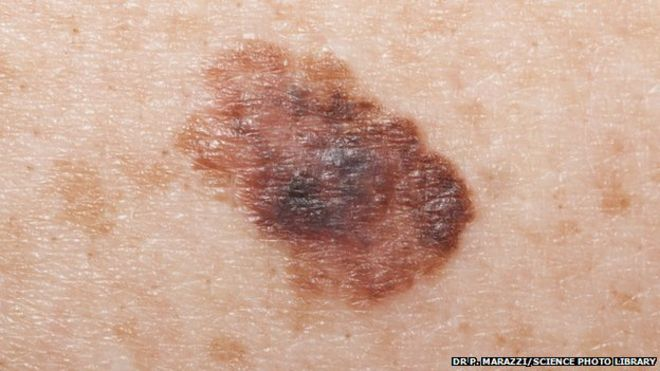
\includegraphics[width=90mm, scale = 0.8]{Figuras/skin_cancer_bbc.jpg}
    \centering
    \caption{Melanoma de piel, Dr. P. Marazzi, Science Photo Library (2012).}
    \label{fig:can_jpg}
\end{figure}


En los últimos años se han logrado muchos avances en cuanto al desarrollo de <<software inteligente>> que han permitido un mayor acceso a diferentes servicios, una de estas tecnologías sería la <<\emph{\gls{rn}}>>, se trata de una tecnología que tiene la capacidad de aprender de los datos históricos mediante el úso de datos históricos y funciones de optimización para crear un modelo matemático capaz de predecir, clasificar o recrear datos futuros o desconocidos. Algunos de los sectores que han mostrado un incremento en el uso de ésta tecnología son: el sector automotriz (piloto automático), el sector de manufactura (optimización de procesos), el sector de entretenimiento (recomendaciones personalizadas), el sector médico (diagnóstico de imágenes). 


\section{Hipótesis}
Es posible clasificar los píxeles en distintas categorías dentro de una imagen gracias a las avances actuales de inteligencia artificial y la técnica de segmentación. Mediante la técnica de \emph{\gls{seg}} es posible crear un reconocedor visual que no solo detecte la presencia y ubicación del elemento a reconocer, sino que, también obtenga otros datos descriptivos del elemento como el tamaño, forma y región que abarca dentro de la imagen. De esta forma se podría obtener un diagnóstico mucho más profundo que permita una detección más acertada.

\section{Objetivos}
Primero en \emph{Objetivo General} se hablará de manera conceptual la problemática a resolver tales como cuales son las situaciones en las que podemos optimizar la resolución de un problema mediante el uso de la tecnología <<deep learning>>, posteriormente en los \emph{Objetivos Específicos} se hablará sobre el objetivo al que queremos llegar utilizando antecedentes de herramientas y teorías de otros experimentos similares para adaptarlo a nuestro problema.

\subsection{Objetivo General}
El \emph{objetivo general} de este experimento es la localización de anomalías en la superficie piel que correspondan a alguno de los tipos de cáncer de esta región (basalioma, carcinoma, melanoma) mediante imágenes, con el uso de la red neuronal de \emph{\gls{seg}} basada en el modelo propuesto por \citeauthor*{wu2019fastfcn} (\citeyear{wu2019fastfcn}), con la finalidad de crear un modelo red neuronal profunda capaz de segmentar de forma semántica las imágenes y sus correspondientes categorías de forma accesible y éficaz. Y de esta forma asistír a los especialistas médicos en su labor de detección y prevención del cáncer de piel.

\subsection{Objetivo Específico}
El \emph{objetivo específico} del experimento es el implementar una red neuronal que primero decodifique una imagen de entrada y extraiga el mapa de características de dicha, y posteriormente reconstruya la imagen remarcando la región donde se encuentra el objeto a localizar. Para esto será necesario dar un recorrido por el proceso de transformación de las dimensiones de la imagen y la arquitectura de la red neuronal requerida para obtener dicho resultado.

\begin{figure}
    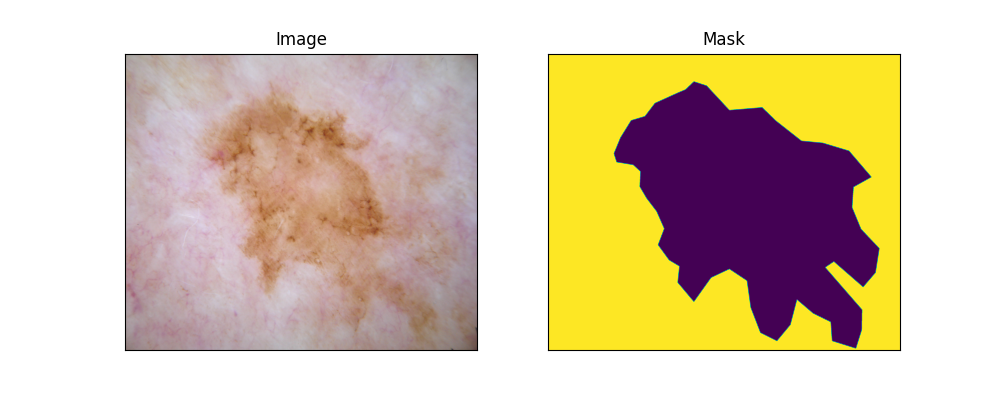
\includegraphics[width=150mm]{Figuras/plot_masks.png}
    \centering
    \caption{Ejemplo de imagen de entrada (izquierda) y resultado esperado (derecha).}
\end{figure}

\section{Estructura de la tesis}

\chapter{Antecedentes}

\chapter{Estado del Arte}

\chapter{Descripción de los datos}

\chapter{Implementación de la Solución}

\chapter{Resultados}

